\fancychapter{Leveraging the \ac{RR} model in distributed storage}\label{chap:storage}
\cleardoublepage{}

% Story 1: bottom-up
%  1. Batching can improve device throughput

%  2. Waiting for batches introduces delays: latency suffers

%  3. We can be eager, reply once the data is in an in-memory
%  buffer

%  4. This introduces a fault-tolerance problem: if the device
%  crashes before the buffer is flushed, the data is lost

%  5. In replicated systems, we can protect against data loss by
%  replying eagerly in some replicas and waiting for data to be
%  in disk in others. If done strategically, it ensures that
%  enough replicas have committed and enough replicas replied
%  fast

%  6. The replicated system needs to tolerate forgetful nodes:
%  if there is a crash and a node loses its soft state it needs
%  to be able to signal that it may be offering stale state back.

%  7. This is exactly the model offered by the restart-rollback
%  model, originally conceived in the context of Trusted
%  Execution Environments with persistent storage.

%  8. This combination is far from trivial. It requires careful
%  adaptations to the storage layer to support different modes
%  of operation and realizing the throughput benefits through
%  batching. At the protocol level, this asymmetry of operation
%  between replicas (with some replying eagerly while others
%  flushing to disk) introduces the challenge of scheduling these
%  sets. This scheduling is crucial to maximize performance, and offers
%  a rich design space.

%  9. Our construction also introduces deployment challenges:
%  the parametrization of the different types of faults the
%  system can suffer is not obvious. We explain how to reason
%  about the reliability and availability of the system to, in
%  conjunction with empirical evidence, derive an adequate
%  deployment for the system requirements.

%  10. Contributions:
%      - Application of a recent fault model to achieve batching
%      throughput benefits without sacrificing safety
%      - The design of a novel storage layer
%      - An exploration of flush scheduling and its impact on
%      throughput and latency
%      - Evidence based parametrization of the resulting system, informed by the
%      desired reliability and availability
%      - PoC implementations and evaluation

% @bsd: problems with the story: I think this misses the whole
% "arc" of persistence in distributed systems, which I think is
% an important contribution

% 1, 2, 3 and 4: the whys, whats and hows of batching
Batching multiple small write operations to a block-oriented storage device into a
single large one is a known mechanism to increase its throughput.
To achieve this batching, one has to wait for an adequate amount
of contiguous data to write, which introduces a delay in the
operation. Alternatively, once the data to write is present in
an in-memory buffer (soft state) the system could return to the
client. This opens the possibility of data loss, if the system
crashes before effectively synchronizing this data to the persistent
storage device.

% 5: replication should be able to partially mask this
%
% note: we can introduce the difference between persistent replicated
% storage systems and volatile replicated storage systems
This problem is propagated as is to current persistent replicated storage
systems: the throughput of the system is limited by the
throughput of the storage devices of the replicas. To avoid this
performance penalty, some replicated systems consider data to be persisted if it is
present in volatile memory at a sufficiently large subset of replicas~\cite{pbft}
(i.e.\ persistence through replication). Such an approach is not
consensual, with other authors insisting that data must be
present in stable storage to be considered persisted~\cite{}.

% Question whether this needs to be a dichotomy
We argue that these two properties --- performance and
durability --- do not need to be mutually exclusive. Instead, we
aim to combine both into a system that offers the throughput from
the solutions which persist in the background with the high
durability from systems which persist before replying to
requests.

% We present a new replication strategy
To this end, we present a novel replication strategy based on
carefully and strategically mixing both approaches, leveraging
\ac{RR} quorum systems. Instead of issuing the write
requests blindly to all replicas, as is costumary, we can
strategically signal to certain replicas to synchronize to
persistent storage before replying while allowing others to
acknowledge the write eagerly, thus mixing both approaches. This
key insight allows us to take advantage of batching, improving the overall
performance of the system, without relinquishing fault tolerance.
The \ac{RR} fault model is needed in case replicas crash before
synchronizing their soft state to stable storage.

% 8, 9: challenges
This approach opens a series of challenges. The storage layer
requires careful adaptations to support multiple modes of
operation the replication protocol needs tap into to orchestrate
the overall system, while offering efficient batching, even on
non-sequential writes. At the protocol level, the asymmetry of
operation between replicas introduces the problem of \emph{sync
scheduling}: choosing which replicas synchronize to persistent storage
and which can reply eagerly. This schedule is paramount to
extracting the maximum performance of the system, and offers a
rich design space. Parametrizing a deployment of such a system is
also not obvious. There is a tradeoff to be explored between the
total number of replicas, the number of replicas which can be
allowed to suffer a rollback (and, by extension, the performance
of the system \bsd{is this immediately clear?}) and the desired
availability and reliability of the system. We present a
principled method for this parametrization, where a system
administrator can tune the number of replicas based on how prone
to faults they are and the desired availability and durability
levels.

\bsd{I feel that some of the key takeaways of these tradeoffs are
missing. This sounds too much as a list of challenges, without
any immediate resolution}

In this chapter, we will present \ac{R2-S2}, a replicated
\ac{KVS} based on LevelDB~\cite{leveldb}, a single node \ac{KVS}
based on \ac{LSM}~\cite{lsm}, where we have implemented several modes
of replication to compare between the different approaches. The
design of the \ac{R2-S2} system is presented in
Section~\ref{sec:r2s2design} and the guidelines for system
parametrization discussed in
Sections~\ref{sec:r2s2parametrization}.
Section~\ref{sec:r2s2implementation} describes the implementation
of the PoC and a preliminary evaluation is presented in
Section~\ref{sec:r2s2evaluation}.

%%%%%%%%%%%%%%%%%%%%%%%%%%%%%%%%%%%%%%%%%%%%%%
\section{\ac{R2-S2} Design}\label{sec:r2s2design}
%%%%%%%%%%%%%%%%%%%%%%%%%%%%%%%%%%%%%%%%%%%%%%

This section presents the design of replicated storage systems
based on the principle of \emph{asymmetric synchronization}. However,
before discussing our architecture in detail, it is worthwhile to
present two baseline designs, which will be useful comparison
points.

\paragraph{Safe but Slow --- SbS.} This architecture relies on
only replying to write requests after writing to persistent
storage. Enabling batching will introduce a large latency delay,
but there is no data loss possible.

\paragraph{Fast but Faulty --- FbF.} Here, replicas reply after
writing to memory. Synchronizing to persistent storage is done in
the background, enabling a very fast system. However, it requires
that a subset of replicas is always up --- otherwise data will be
permanently lost.


We now present the principles and goals for our design:
\begin{enumerate}
    \item \textbf{Strong Persistence}: data loss should never
        ocurr, even in the presence of arbitrary node crashes;

    \item \textbf{Performance}: the architecture should yield
        performance gains compared to SbS\@;

    \item \textbf{Generality}: the architecture should be as
        generic as possible. In particular, it should be
        applicable to a variety of replication protocols.
\end{enumerate}

Note that none of our baselines satisfy all requirements.
Although both are generic, the FbF architecture fails our notion
of \emph{strong persistence}: if enough replicas crash before
writing to persistent storage, data is lost. Similarly, the SbS
architecture is overly cautious when writing to persistent
storage, failing our performance goal.

In the remainder of this section, we will describe
\emph{asymmetric synchronization}, the key technique which realizes the
goals prescribed above, and how the architecture needs to
acommodate this paradigm to achieve the best possible
performance.

%%%%%%%%%%%%%%%%%%%%%%%%%%%%%%%%%%%%%%%%%%%%%%
\subsection{Asymmetric Synchronization}\label{ssec:asymmetric_synchronization}
%%%%%%%%%%%%%%%%%%%%%%%%%%%%%%%%%%%%%%%%%%%%%%

Asymmetric synchronization works by separating the replica set
into two disjoint subsets: the \emph{volatile set}
$\mathbbm{r}$, composed of the replicas which eagerly reply to the
request (before synchronizing to persistent storage); and the
sync set $\mathbb{F}$, the replicas which wait until the data is
persisted before replying. The intersection between a write
quorum $\mathbb{W}_Q$ and the sync set is the \emph{critical
sync set}. When issuing a write request, each replica is told in
which set they belong to, and act accordingly.

\paragraph{Achieving strong persistence.} To achieve strong
persistence, it is sufficient that the critical sync set is
never null. This implies that there is always at least one
replica in every write quorum which persisted the value, making
it recoverable. This is guaranteed by the restart-rollback quorum
system, by setting the maximum size of $\mathbbm{r}$ to $r$,
since the volatile replicas are the ones which can suffer the rollback on
restart, and as such the volatile set size must never exceed $r$.

\paragraph{Extracting performance.} To minimize latency and
maximize throughput, we further separate the write behaviour
within replica set. In particular, the critical sync set
operates differently from its non-critical counterpart. This is
because the critical sync set is the limiting latency factor
within a single operation, and as such should write to persistent
storage immediately. The non-critical sync set can wait until it
has an adequately sized batch to synchronize. The storage layer needs
to support both use-cases efficiently.

The key to improving throughput is precise scheduling. By
choosing different eager, critical sync and non-critical sync
sets, we can guarantee that when a replica is in the critical sync set it
has enough data queued in memory, amortizing the persistent
access cost.

Compared to SbS, this construction can yield throughput or latency benefits,
depending on how the the tradeoff is tuned in SbS --- if SbS writes to
persistent storage immediately, our design provides a throughput
improvement; if SbS waits for a batch, our design provides better
latency. Regretablly, it is impossible to match the performance
of FbF\@: this would require removing any persistent accesses from
the critical path, making $\mathbb{W}_Q \cap \mathbb{F} =
\varnothing$, violating strong persistence.


%%%%%%%%%%%%%%%%%%%%%%%%%%%%%%%%%%%%%%%%%%%%%%
\subsection{Storage Layer}\label{ssec:storage}
%%%%%%%%%%%%%%%%%%%%%%%%%%%%%%%%%%%%%%%%%%%%%%

The storage layer plays a crucial role in realizing the
performance potential of the system. It needs to efficiently support
three different types of write operations --- eager, immediate
sync and delayed sync. It will also need to support read operations
efficiently. Figure~\ref{fig:storage_layer} shows a diagram of
the storage layer and its data-structures.

An LSM is employed as the core data structure of the storage
layer, enabling the sequential writes required for batching as
well as providing reasonable read performance.

To further speed up reads and enable batching, there is an in-memory
object cache. Values are marked \emph{dirty} if they have not yet been
written to persistent storage (because they are waiting to be
included in the next batch). Although the cache is organized as a
table to support fast reads, the dirty values form a linked list,
to avoid duplication and guaranteeing quick access when it is
time to create a batch.

There is an additional in-memory cache, which only stores the
object versions. This is useful because versions are a staple of
most replication protocols and several of them require reading
the current version before writing a new one. Since versions are
constant-sized and small, the capacity of the version cache can
be significantly larger than that of the object cache.

Satisfying read requests is trivial: the appropriate cache is
consulted (depending on whether it is an object or a version
read), falling back on the LSM tree in the event of a miss.

Handling volatile writes and delayed synchronized writes is remarkably similar: the
value is placed in the in-memory cache and marked dirty by
linking it into the linked list. They differ by when the write is
actually externalized: the volatile write returns after the cache
write; the delayed synchronized write waits for the value to be
synchronized to the LSM tree. When handling an immediate
synchronized write, the value is
placed into a fresh batch and elements are popped from dirty
object linked list until the batch is large enough, at which
point it is committed to the LSM tree and the immediate synchronized write
returns (as well as any delayed synchronized writes which were included
in the batch).

Note that if the dirty object linked list is large enough
for two batches, a single batch could be created and committed.
This would still leave enough elements to create a batch in the
event of an immediate synchronized write of a small object. However, if
two such writes arrived, we would have to synchronize a write without
ammortization, losing throughput. As such, we delegate all
synchronization decisions to the schedule.

\bsd{It pains me to say, but a god-forsaken ML-based scheduler
would be a great fit. This is because the size of writes weighs
heavily on the schedule, but cannot be known ahead of time.
However, an reinforcement learning network would adapt to traffic
as it came\ldots. We can also make the schedules conditional on
the size of the object, but this becomes very difficult}

\begin{figure}[ht]
    \centering
    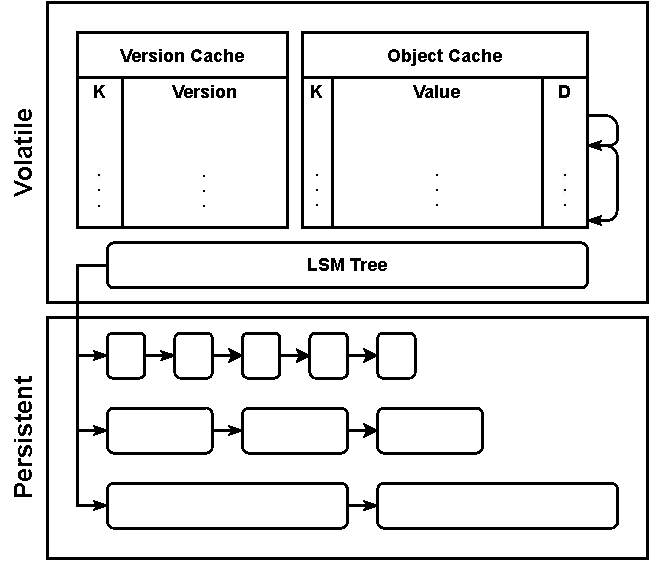
\includegraphics[width=.8\linewidth]{img/storage_layer}
    \caption{Diagram of the Storage Layer}\label{fig:storage_layer}
\end{figure}

\bsd{Possible speedup: on version cache miss, we could just read
the beginning of the log entry, if we serialize the version at
the head of the object}

%%%%%%%%%%%%%%%%%%%%%%%%%%%%%%%%%%%%%%%%%%%%%%
\subsection{Scheduling}\label{ssec:schedule}
%%%%%%%%%%%%%%%%%%%%%%%%%%%%%%%%%%%%%%%%%%%%%%


As we have covered, a good schedule is crucial to realize the
performance potential of the architecture. A \emph{schedule} for
replica $i$, $S_i$ is a sequence of modes of operation (eager,
immediate sync or delayed sync) which the replica will follow.
We call the set of replica schedules the \emph{system schedule}.
We say that the system schedule is \emph{valid} if the size of
volatile set for each operation is less than or equal to $r$. All valid
schedules guarantee strong persistence, but this is not enough to
ensure performance. The \emph{scheduler} is the module that
generates a schedule.

\subsubsection{Approaches to scheduling}\label{sssec:scheduling_approach}

There are several approaches to scheduling. Which is preferable
is non-obvious beforehand: the schedule will be sensitive to the
particularities of the replication protocol, the deployment and
the operation load. In the preliminary evaluation in
\S~\ref{sec:r2s2evaluation} we present an
evaluation of some of the scheduling policies described
here.

\paragraph{Static Schedules.} These schedules apply a fixed
policy decided beforehand, irrespective of the runtime
characteristics of the system. Such a schedule can be
\emph{blind} or \emph{informed}, depending on whether it uses
deployment information or not (eg: network topology, hardware
specification). Examples of blind schedules: \emph{random}
schedule, \emph{round-robin} schedule.

\paragraph{Dynamic schedules.} Information reported by the
replicas (eg: storage layer performance, amount and size of dirty
objects, network behaviour, detected/suspected faults) is used by
the scheduler to constantly adapt to create the best schedule
possible. A dynamic scheduler can be implemented using
SMT solvers~\cite{smt} or a neural network. \bsd{develop}

In the case of dynamic schedules, the performance of the
scheduler can be of importance. To understand why, it is
important to distinguish between \emph{ahead-of-time} (AoT) and
\emph{just-in-time} (JIT) schedulers.

An AoT scheduler will compute several entries of the schedule beforehand. When a
request arrives, it simply consults the schedule. If the schedule
is close to finishing or new information arrives, the scheduler
can compute or recompute schedule entries in the background.
However, these schedulers suffer from a major problem: the size
of the objects to be written is unknown ahead of time (although
it can possibly be predicted, studying the history).

The size of the object is crucially important for performance, as
it will impact whether the critical sync set replicas have
enough data to form a batch or not. By employing a JIT, we can
factor in the object size when creating the schedule.
Nevertheless, the scheduler now sits on the critical path of the
write operation: if it takes too long to generate the schedule,
it risks destroy any possible performance gains it would achieve.

\bsd{there is more to be said about this topic\ldots}

\subsubsection{Computing and executing schedules}\label{sssec:schedule_computation}

Up until this point we have been describing the scheduler as if
it is centralized, with perfect information. This can at times
closely match practice: in leader-based protocols, the scheduler
is collocated with the leader. All replicas monitor their own
performance and communicate it periodically to the leader
(possibly piggybacking this information with operation replies).

In leaderless protocols, this is unfortunately impossible, as it
is the clients which need to compute and execute the schedule.
Even if somehow a client could compute (or obtain) the schedule,
in the event of concurrency client synchronization would be
required to correctly execute the schedule. This synchronization
would be expensive (if not outright impossible).

To sidestep this issue, in leaderless protocols there is a
separation of responsibilities regarding the schedule: the
clients are responsible for \emph{computing} the schedule and
replicas simply \emph{execute} it. When a fresh client makes it
first request (employing blind scheduling), the replicas might
ignore the schedule transmitted by the requests \emph{if they
have a previous schedule installed}. If they do not, they accept
the scheduling suggestion and relay back their monitoring
information. With this, the client can then compute a schedule
and install it to the replicas.

Figure~\ref{fig:replica} shows an overview of the scheduling
architecture within a replica.

\begin{figure}[ht]
    \centering
    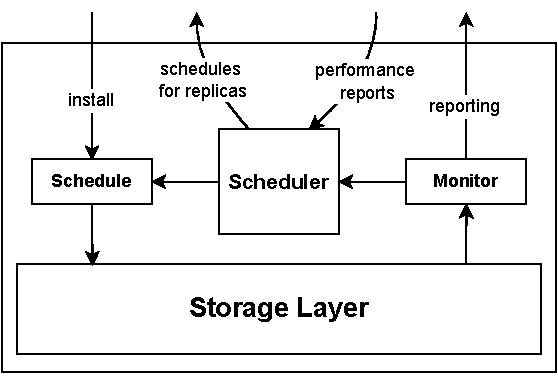
\includegraphics[width=.8\linewidth]{img/replica}
    \caption{Replica scheduling architecture. A monitor is attached to
    the storage layer, measuring its performance and passing that
    information either to the local scheduler or to other
    replicas/clients. If the replica is a leader, the scheduler
    collects performance reports and creates schedules for itself
    and other replicas. Otherwise, it simply uses the installed
    schedule.}\label{fig:replica}
\end{figure}

\bsd{Ommitted notes: a schedule installation requires SMR, to
make sure all replicas install the same schedule in the event of
concurrent clients}

\bsd{Unsolved problem: request reordering/loss. This can
make the decentralized schedule execution invalid.
\\
\\
Idea: have per-client schedules. This involves having separate
dirty lists per client, load-balancing between clients and some
sort of orphan collection}

%%%%%%%%%%%%%%%%%%%%%%%%%%%%%%%%%%%%%%%%%%%%%%
\section{Parametrizing the System}\label{sec:r2s2parametrization}
%%%%%%%%%%%%%%%%%%%%%%%%%%%%%%%%%%%%%%%%%%%%%%

To parametrize our system, we effectively need to choose
appropriate values for $r$ and $f$. We employ a data-driven
approach to this problem. Relying on real-world information about
the availability and reliability of components, we can predict
the reliability and availability of the system as a function of
$r$ and $f$. Choosing the adequate values becomes an exercise of
setting the desired reliability/availability and solving for $r$
and $f$.

The availability of the system (probability that it is available
at a particular point in time) is impacted by the availability of
the individual replicas. Let $p_c$ be the symmetric of the
availability of a replica, ie: the probability that a replica is
\emph{crashed} at a particular point in time.

The reliability (probability that the system loses data) of the
system is dependent on the reliability of the underlying storage
devices and the availability of the replicas in the eager set.
Let $p_f$ be the probability that a storage device fails
(irrecoverably).

These metrics will also be deployment sensitive. Let us consider
that the replicas are geo-replicated. In this scenario, replica
crashes are not correlated, and as such the probability that an
eager set crashes at the same time is $p_c^r$. Now let us imagine
that all replicas are within a single datacenter. Here if a
replica crashes it is highly likely that the others also crashed
(eg: the crash was caused by a power outage), meaning that the
probability that the eager set crashes is still $p_c$.

Table~\ref{tab:parametrization} summarizes the availability and
reliability of the system in these two scenarios.

\begin{table}[ht]
    \centering
    \caption{Availability and reliability in a geo-replicated
    deployment versus a datacenter deployment. $R_Q$ and $W_Q$
    are the sizes of the quorums for a parametrization with $M_R$
    tolerated rollbacks and $F$ crash faults}\label{tab:parametrization}
    \begin{tabular}{|r||c|c|}
        \hline
        & \textbf{Geo-replicated} & \textbf{Datacenter} \\ \hline
        \textbf{Availability} & $1 - p_c^{\min(R_Q, W_Q)}$ & $1 - p_c$ \\ \hline
        \textbf{Reliability}  & $1 - p_c^{M_R} \cdot p_f^{W_Q - M_R}$ & $1 - p_c \cdot p_f^{W_Q - M_R}$ \\ \hline
    \end{tabular}\label{tab:parametrization}
\end{table}


%%%%%%%%%%%%%%%%%%%%%%%%%%%%%%%%%%%%%%%%%%%%%%
\section{Implementation}\label{sec:r2s2implementation}
%%%%%%%%%%%%%%%%%%%%%%%%%%%%%%%%%%%%%%%%%%%%%%

\bsd{TODO}

%%%%%%%%%%%%%%%%%%%%%%%%%%%%%%%%%%%%%%%%%%%%%%
\section{Evaluation}\label{sec:r2s2evaluation}
%%%%%%%%%%%%%%%%%%%%%%%%%%%%%%%%%%%%%%%%%%%%%%

\bsd{TODO}
